%-------------------------------------------------------------------------------------------
%	Introduction to Writing
%-------------------------------------------------------------------------------------------
\section{Motivation}

% The text appearance and the thesis layout is sometimes determined by formal requirements. This text, for example is \NOTE{Times} using 11pt size and a slight increase in space between the text lines. There are also requirements for indenting a new paragraph sometimes.\\
% As you can see, this template does not indent the new paragraph. However, you can always change this setting in the \NOTE{declarations.tex} file.\\
% \ThinHRule

% Some faculties require to include all references to external sources in \NOTE{footnotes}.\footnote{ This is a footnote. You can also include citations and many text formatting LaTex commands.}\footnote{ You may also explain background information on a topic, which may be interesting for further reading.}\footnote{ Footnotes also often include weblinks, for example \url{http://www.jankuester.com}}\\
% \ThinHRule

% You can enumerate or list some points and sketches of a topic using \NOTE{list or enumerattions}:

% \begin{enumerate}
% 	\item Start
% 	\item Work
% 	\item Finish
% \end{enumerate}


%-------------------------------------------------------------------------------------------
%	Structure of the thesis
%-------------------------------------------------------------------------------------------
\section{Brief History}

\subsection{Language Models: BERT}
Since the current template is structured into chapters, sections and subsections. This is mainly because a master thesis may easily grow up to 100 pages and in some cases even bigger. Structuring your big parts into \NOTE{chapters} makes it perfect for separating in logical units, such as:

\begin{itemize}
	\item Introduction
	\item Related Work
	\item Research Design
	\item Proceedings and Data Collection
	\item Data Analysis and Evaluation
	\item Discussion and Conclusion
\end{itemize}
\ThinHRule

The next smaller units are \NOTE{sections} which structure a chapter into it's subtopics. Using \NOTE{subsections} allows to cover these topics step by step and keep the reader on track with a mental model of all the parts of the current topic.\\
\ThinHRule

Now there are also \NOTE{subsubsections} available in LaTex. It would become very confusing when even \NOTE{including subsubsections in the table of contents (toc)}. For this reason, the toc is set to remove these subsubsections. You may alter this by taking a look into the main.tex and the declaration.tex. 
\ThinHRule

\subsubsection{\textcolor{SECTION_COL}{This Subsubsection is not listed in the Table of Contents}}

The advantage is, that your work becomes more structured along the complexity of your topic. It may occur, that topics can become very granular, which is why this is the perfect counterpart for this issue.

\subsection{Language Models: GPT-3}


\section{Principles of Operation}

In the \NOTE{declaration.tex file}, there is a shorthand command called \NOTE{NOTE}.
Diagrams

\section{Mathematical Formulation}

\newpage
\section{Implementations}
\subsection{Pre-trained Models}

\section{Computational Constraints}

Including a graphics is not that hard. Important is to wrap it as a figure, so that it will be included into the \NOTE{ list of figures}. You can also \NOTE{label} it, which allows to refer directly to this figure without the need of keeping track of it's id or name. Another handy parameter is the \NOTE{width} parameter, which allows to set the dimensions according to the current text width.

\begin{figure}[H]
\begin{center}
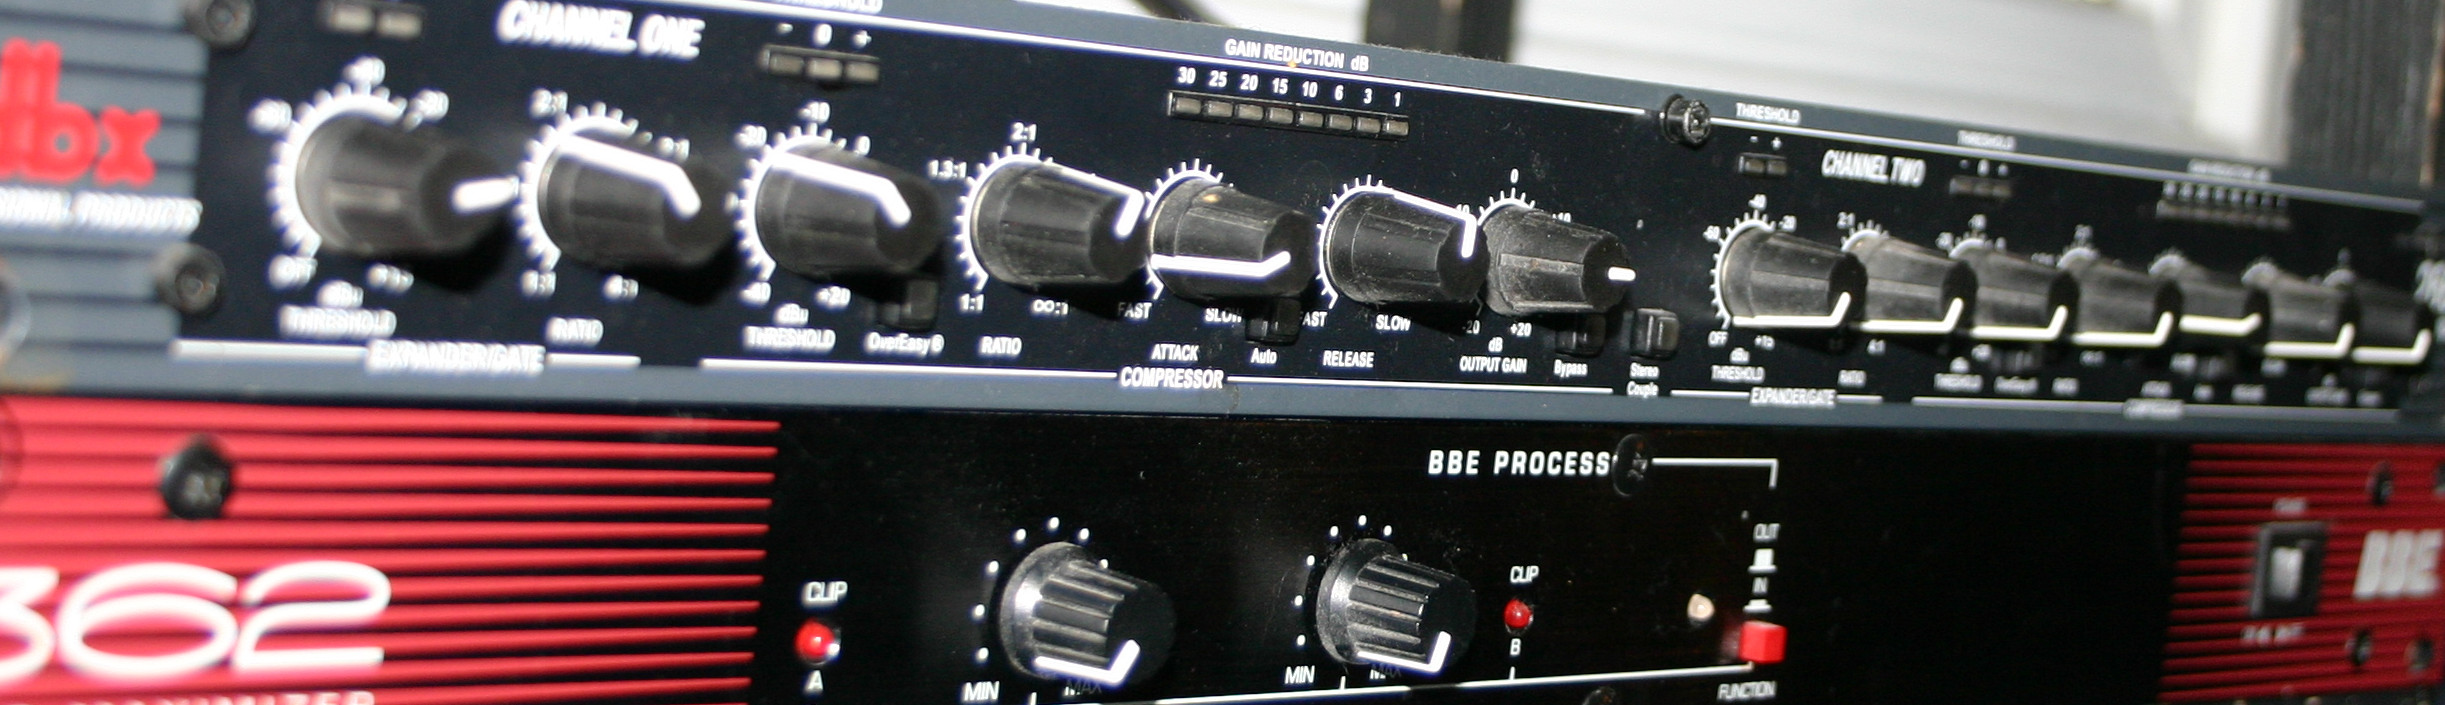
\includegraphics[width=0.8\textwidth]{media/amp.jpg}
\end{center}
\caption[TBC]{description of the figure. }
\end{figure}







